\documentclass[../main.tex]{subfiles}

\begin{document}
    \section{Standard Model of Particle Physics}

    The Standard Model (SM) of particle physics is a framework which contains our current understanding of the matter and three of the four four forces found in the universe. Within the SM there are 12 elementary fermions, 
    5 vector bosons which mediate the three fundamental forces and a scalar boson responsible for particle masses (Figure \ref{fig:SM}). It is important to note that the SM is not a complete model of the universe. A great example of this is the gravitational force 
    which is not described by the theory, however at the small scales of of particle physics this force is neglected due to it's insignificant strength when compared to the other three forces (strong, electromagnetic and weak).
    \begin{figure}[H]
        \centering
        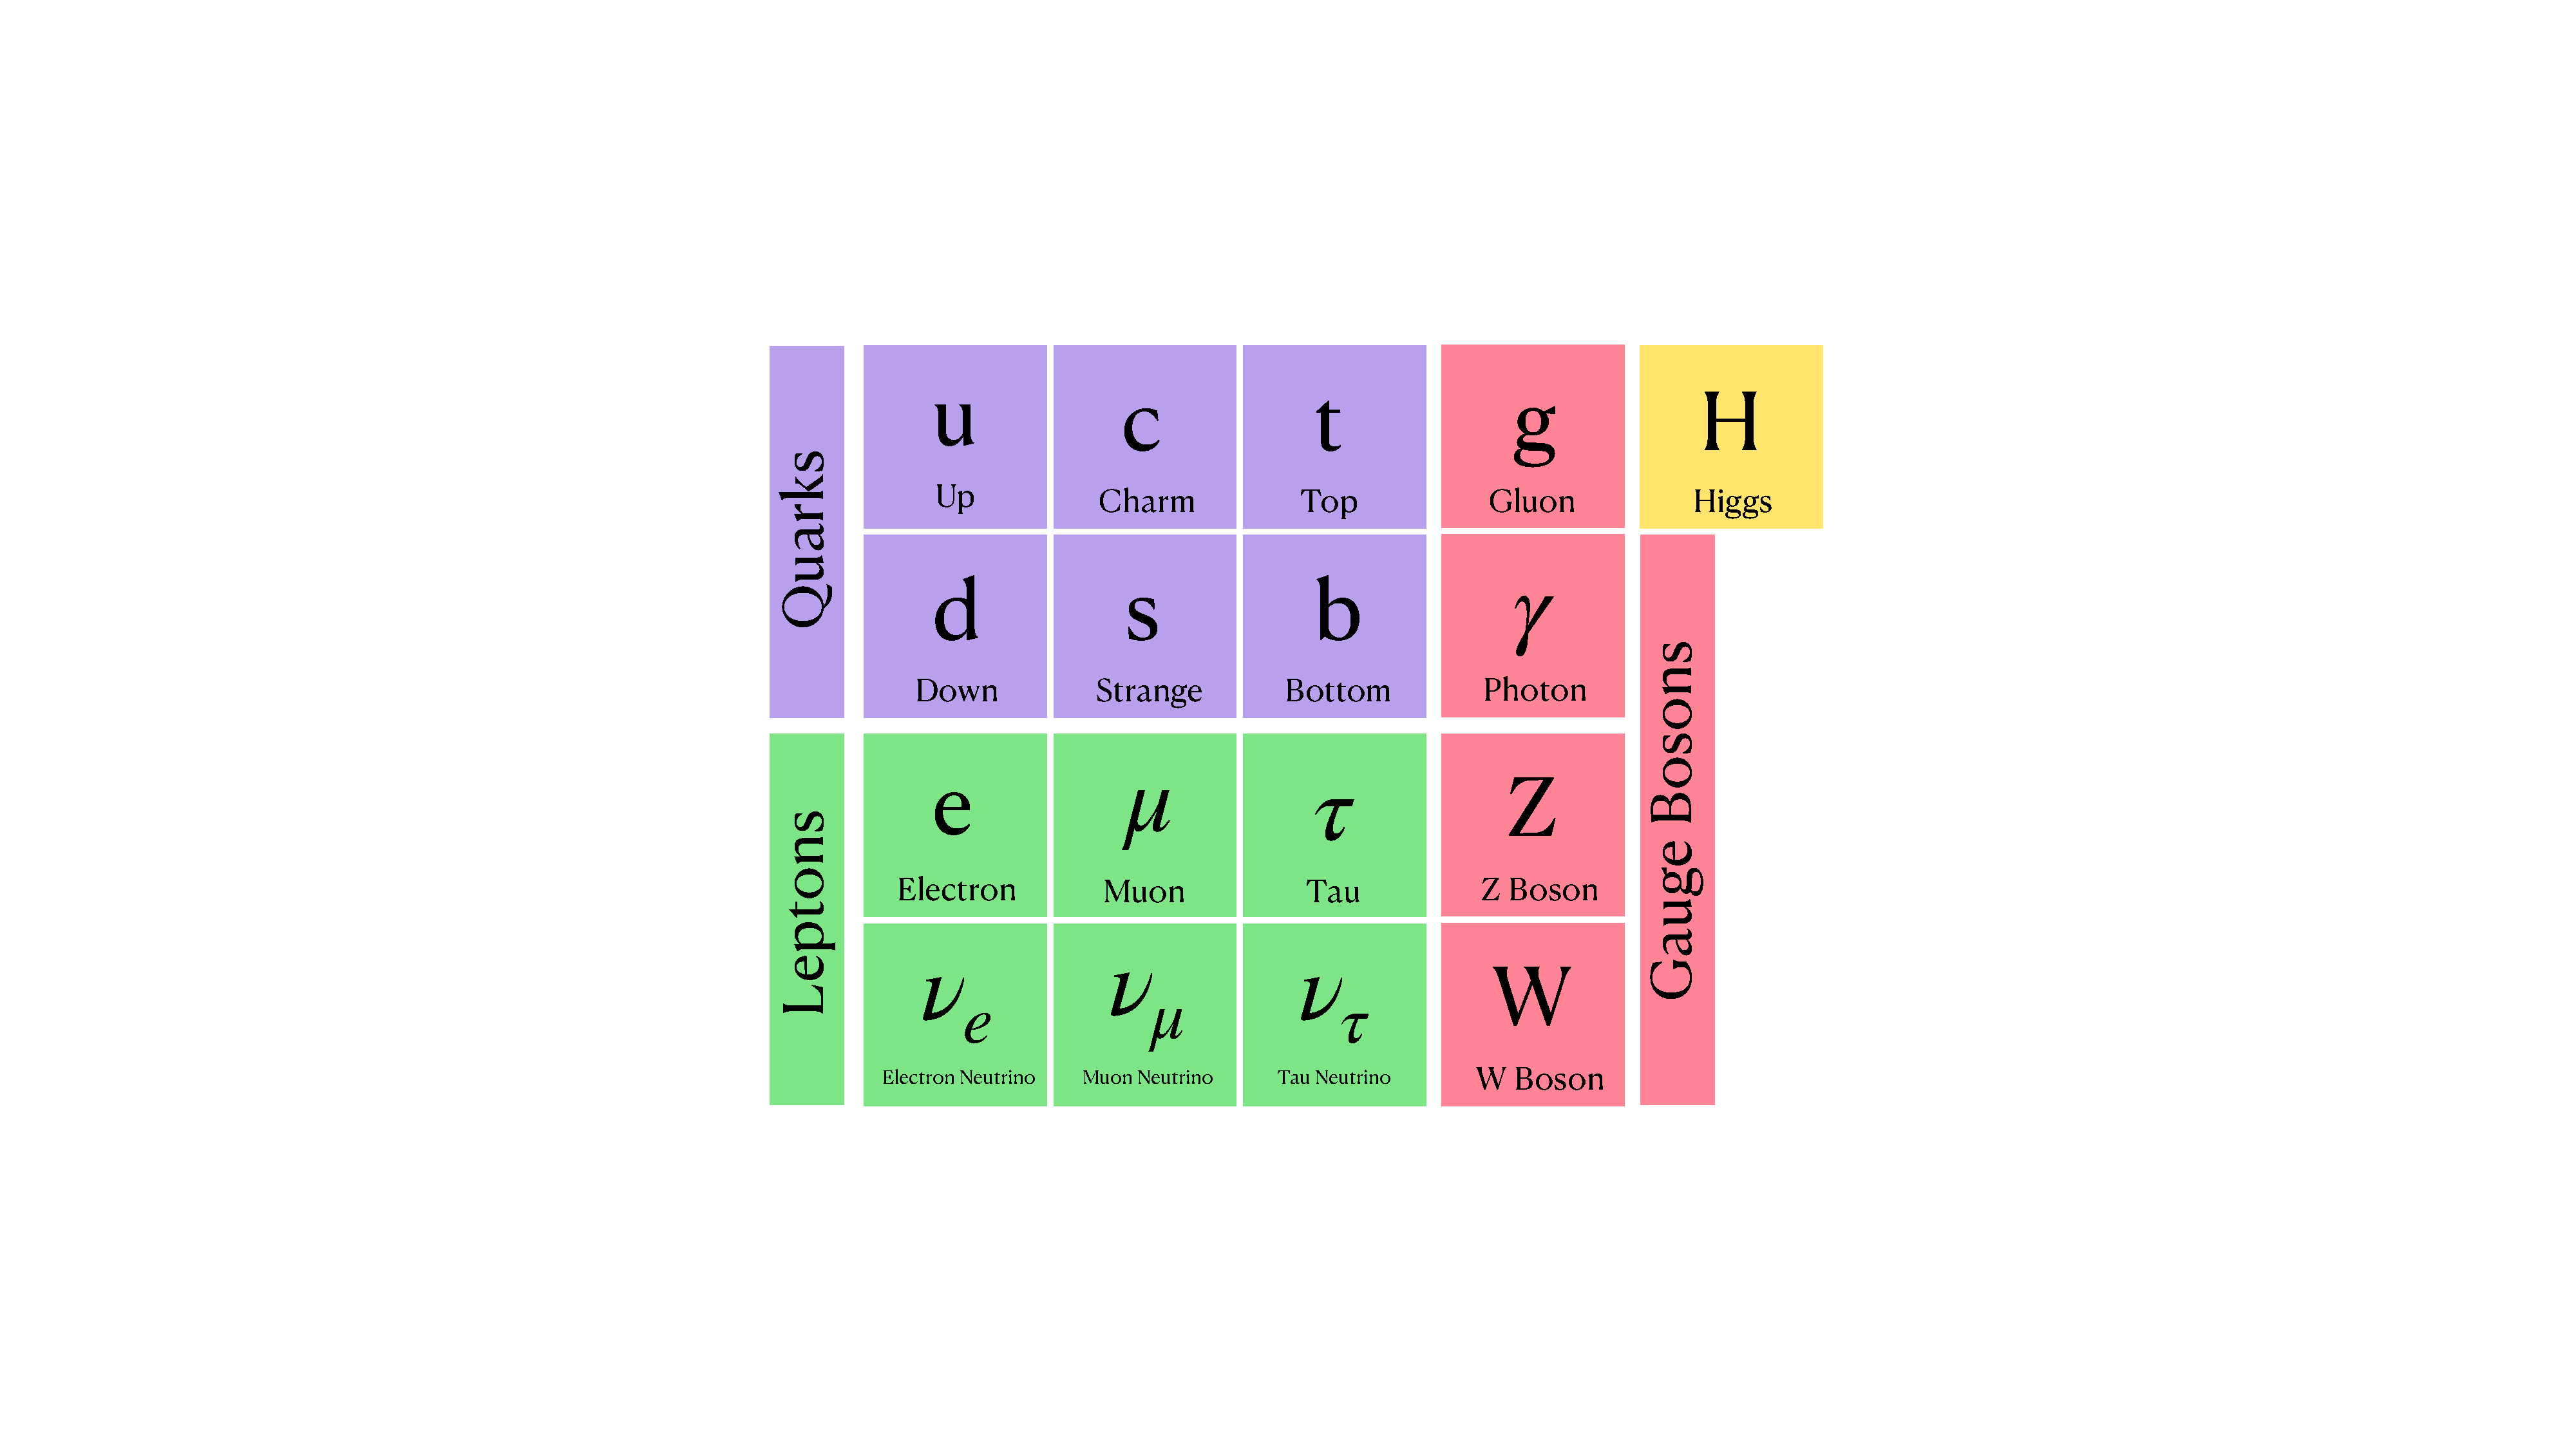
\includegraphics[width=0.7\textwidth]{imgs/SM.pdf}
        \caption{The Standard Model of particle physics with the 12 fermions shown in purple and green, the five vector bosons shown in red and the Higgs scaler boson shown in yellow.}%
        \label{fig:SM}%
    \end{figure}
    The SM comprises of a quantum field theory (QFT) and is based on the non-Abelian gauge symmetry groups SU(3)×SU(2)×U(1). The SU(3) governs the strong interactions and the SU(2)×U(1) the electroweak interactions. 
    Each group contains their respective gauge bosons: gluon for the strong and W,Z and photon for the electroweak. The SU(3) is an exact gauge symmetry where as the electroweak symmetry is spontaneously broken by the Higgs field, resulting 
    in the massive electroweak bosons ($W^{\pm}$ and $Z^{\pm}$). Due to this broken symmetry which gives rise to massive quarks, the strong and weak eigenstates diverge. The weak eigenstates (d', s', b') of down, strange and bottom quarks which are associated to the weak interaction are related to the mass
    eigenstates (d, s, b) through the Cabibbo-Kobayashi-Maskawa (CKM) matrix $V_{\text{CKM}}$ \cite{PhysRevLett.10.531,10.1143/PTP.49.652}. 
    \begin{equation}
    \begin{pmatrix} d' \\ s' \\ b' \end{pmatrix} =
        V_{\text{CKM}}
        \begin{pmatrix} d \\ s \\ b \end{pmatrix} = 
        \begin{pmatrix} 
            V_{ud} & V_{us} & V_{ub} \\ 
            V_{cd} & V_{cs} & V_{cb} \\ 
            V_{td} & V_{ts} & V_{tb} 
        \end{pmatrix}
        \begin{pmatrix} d \\ s \\ b \end{pmatrix}
    \end{equation}

    \ifSubfilesClassLoaded{%
    \bibliographystyle{ieeetr}
    \bibliography{../../references.bib}%
    }{} 
\end{document}